\documentclass{standalone}
\usepackage{xcolor}
\usepackage{tikz}
\usetikzlibrary{datavisualization.formats.functions}

\begin{document}
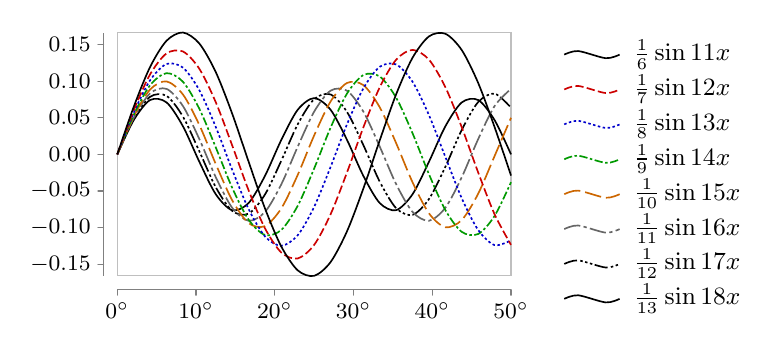
\begin{tikzpicture}
\tikzdatavisualizationset {
  example visualization/.style={
    scientific axes=clean,
    y axis={ticks={style={
          /pgf/number format/fixed,
          /pgf/number format/fixed zerofill,
          /pgf/number format/precision=2}}},
    x axis={ticks={tick suffix=${}^\circ$}},
    1={label in legend={text=$\frac{1}{6}\sin 11x$}},
    2={label in legend={text=$\frac{1}{7}\sin 12x$}},
    3={label in legend={text=$\frac{1}{8}\sin 13x$}},
    4={label in legend={text=$\frac{1}{9}\sin 14x$}},
    5={label in legend={text=$\frac{1}{10}\sin 15x$}},
    6={label in legend={text=$\frac{1}{11}\sin 16x$}},
    7={label in legend={text=$\frac{1}{12}\sin 17x$}},
    8={label in legend={text=$\frac{1}{13}\sin 18x$}}
  }
}
\tikz \datavisualization data group {sin functions} = {
  data [format=function] {
    var set : {1,...,8};
    var x : interval [0:50];
    func y = sin(\value x * (\value{set}+10))/(\value{set}+5);
  }
};
\datavisualization [
  visualize as smooth line/.list=
{1,2,3,4,5,6,7,8},
  example visualization,
  style sheet=strong colors,
  style sheet=vary dashing]
data group {sin functions};
\end{tikzpicture}
\end{document}
